\documentclass[xcolor=x11names]{article}


\usepackage{amsmath}
\usepackage{amsthm}
\usepackage{amssymb}
\usepackage{amsfonts}
\usepackage{graphicx}
\usepackage{caption}
\usepackage{subcaption}
\usepackage[usenames,dvipsnames]{xcolor}
\usepackage{cite}


\newcommand{\degree}{\ensuremath{^\circ}}

%\usepackage{fullpage}

\DeclareGraphicsExtensions{.eps,.pdf,.png,.jpg}


\title{Report on Lab 1}
\author{Tsang-Kai Chang}
\date{\today}
%\date{Sept. 28, 2016}


\begin{document}

\maketitle

\begin{abstract}
abstract
\end{abstract}


%%%%%
\section{Introduction}

   In this lab, I am going to model the most sophisticated physical kinematic linkage: human left arm. To simplify the problem, we consider the shoulder joint (glenohumeral joint) and the elbow joint only, and assume that the wrist joint and all the joints in hand fixed. The left arm connects to the torso on the shoulder joint. The shoulder joint and the elbow joint is connected by the humerus. From the elbow joint, there are two bones connected to the hand: radius and ulna.
   
   
      [picture needed]

   
%%%
\subsection{Modeling}





\begin{figure}
    \centering
    \begin{subfigure}[b]{0.4\textwidth}
        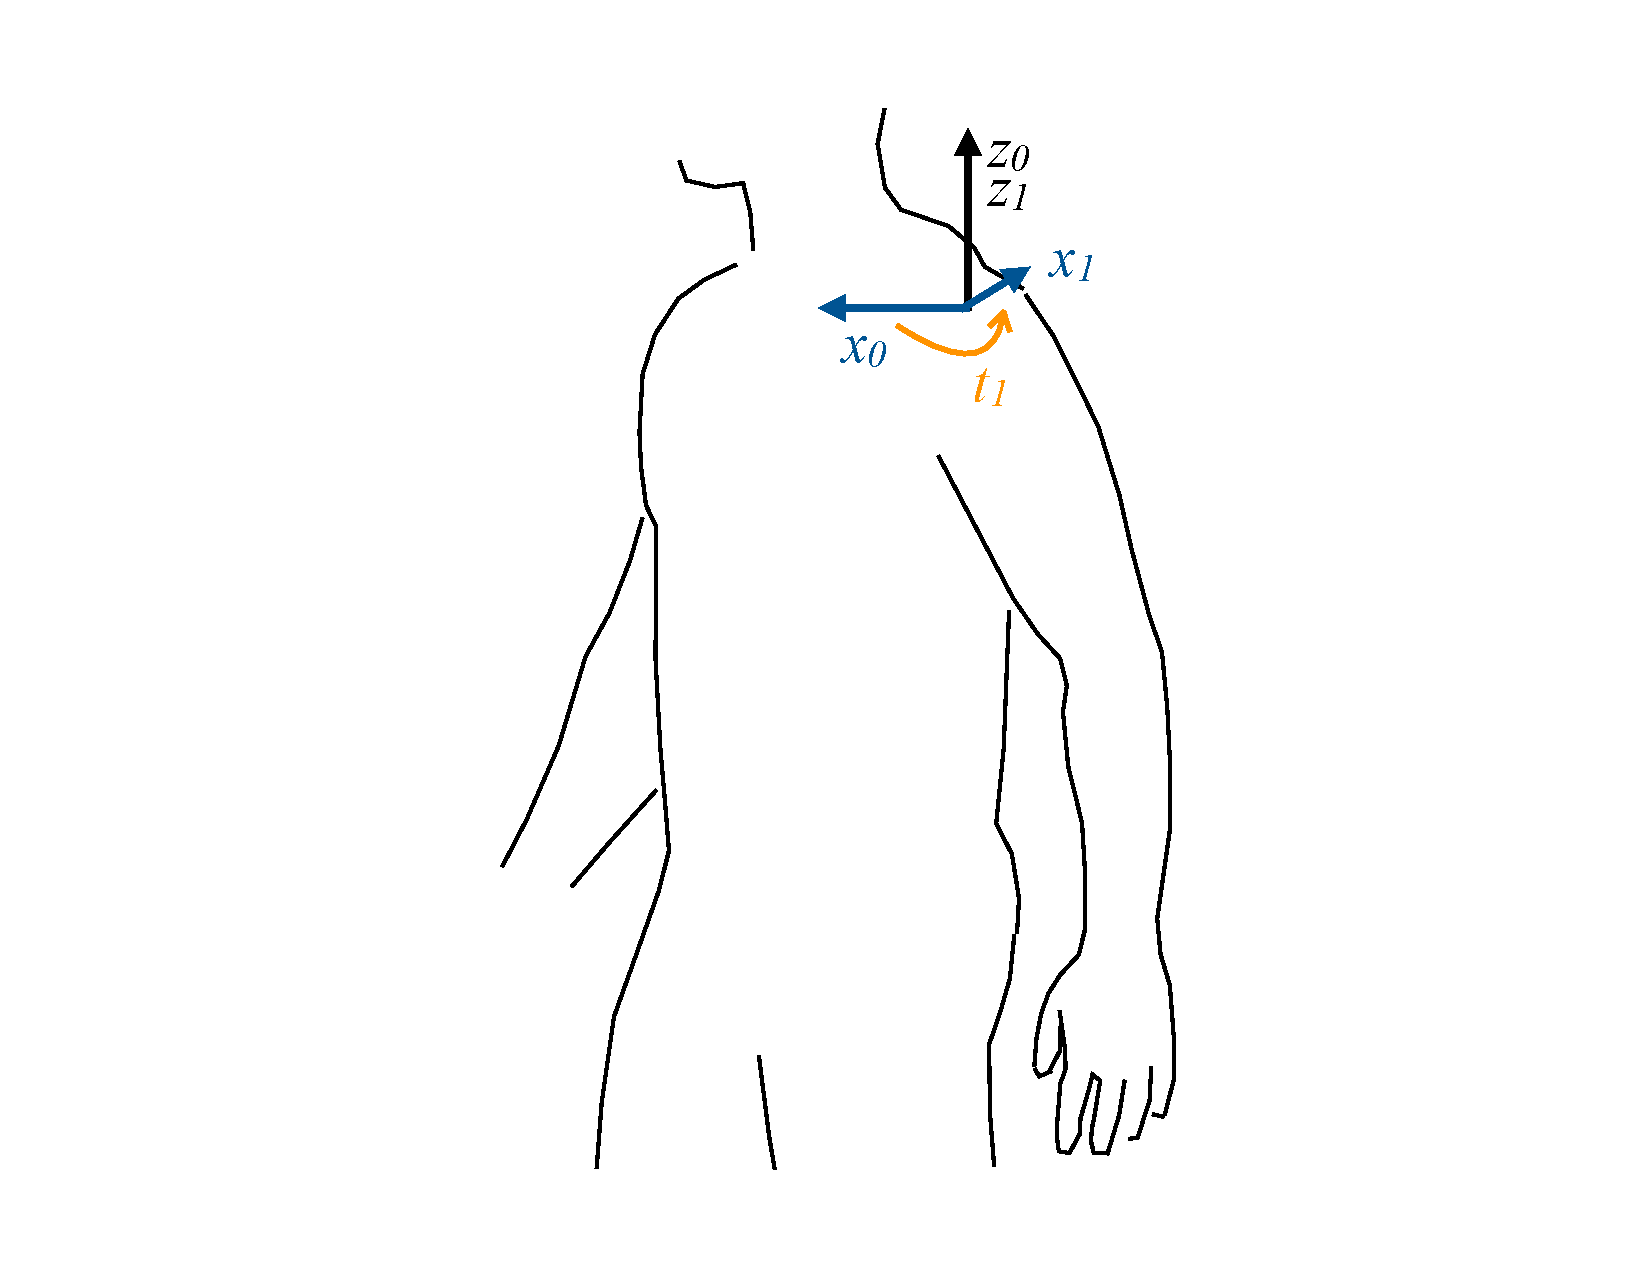
\includegraphics[trim = 50mm 0mm 50mm 0mm, clip, width=\textwidth]{model_1}
        \caption{}
    \end{subfigure}
    ~ %add desired spacing between images, e. g. ~, \quad, \qquad, \hfill etc. 
    \begin{subfigure}[b]{0.4\textwidth}
        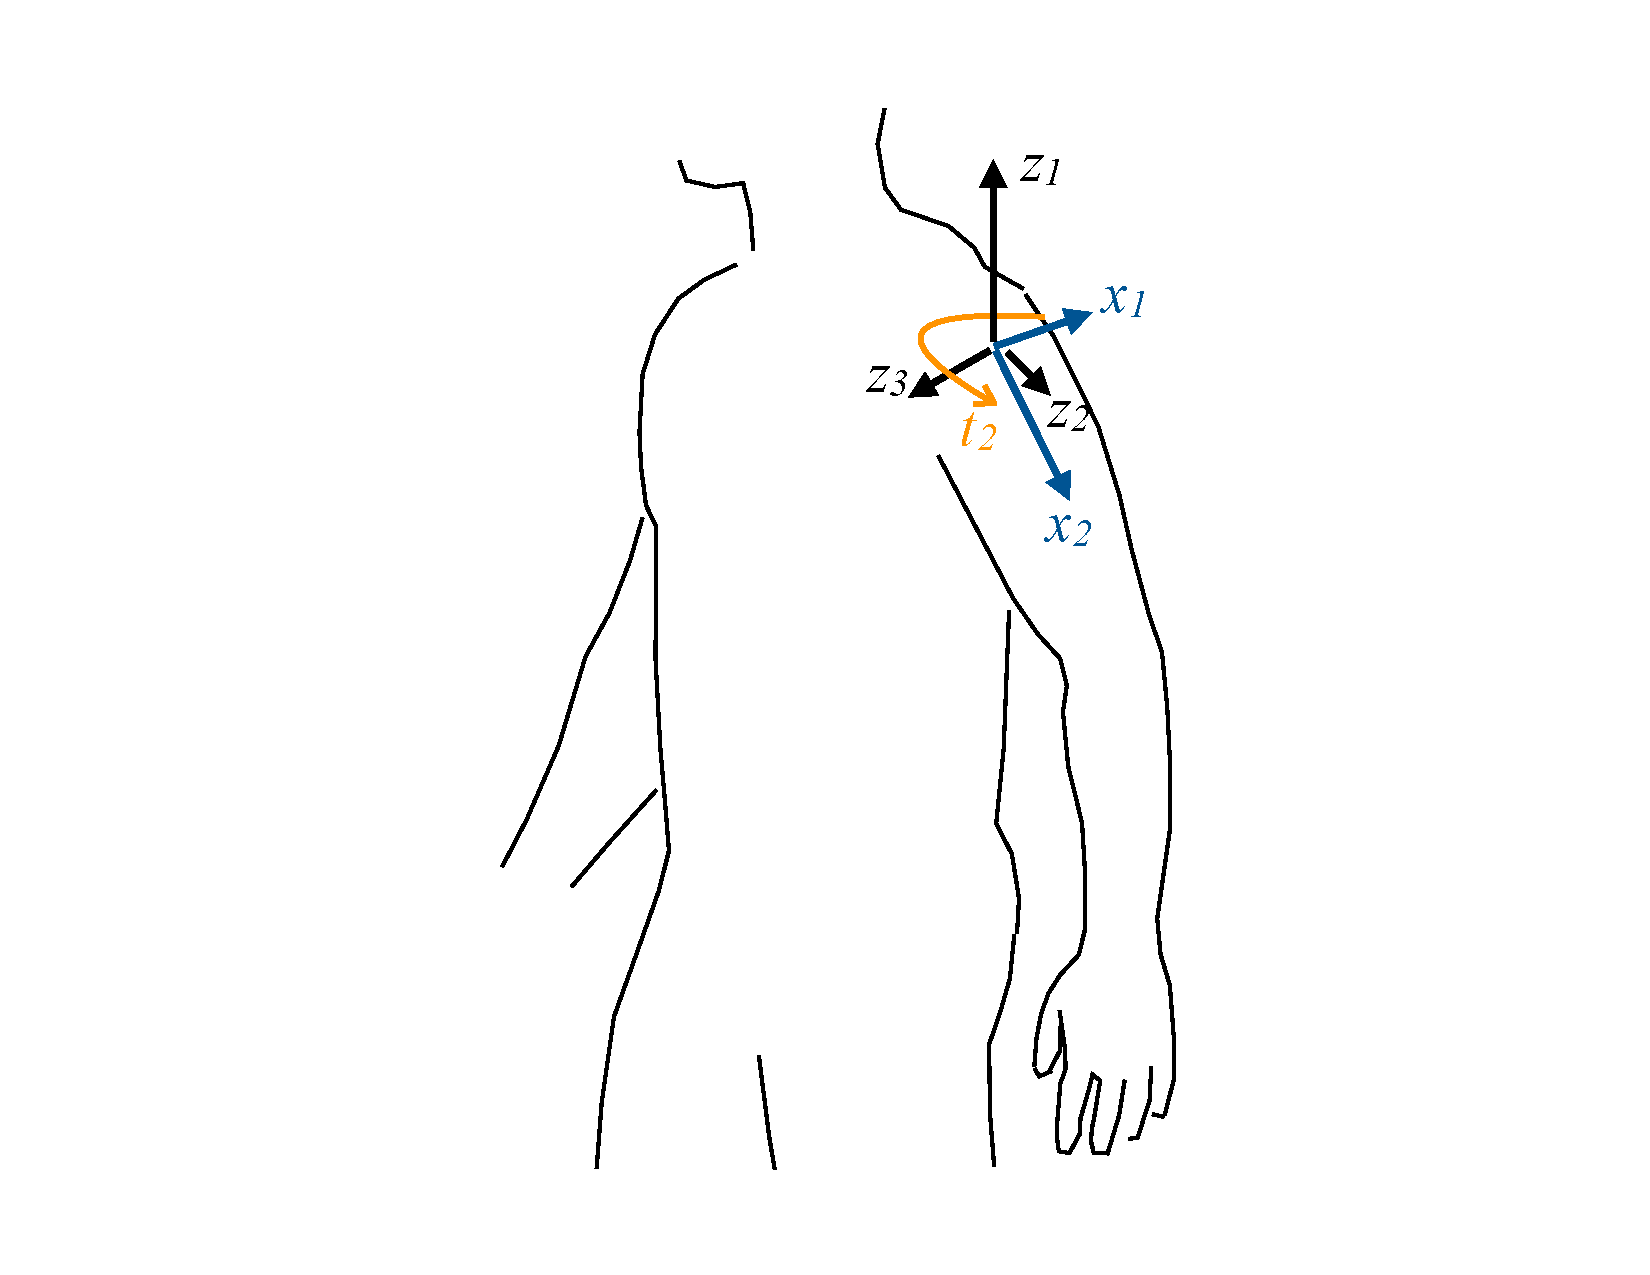
\includegraphics[trim = 50mm 0mm 50mm 0mm, clip, width=\textwidth]{model_2}
        \caption{}
    \end{subfigure}
    \\ %add desired spacing between images, e. g. ~, \quad, \qquad, \hfill etc. 
    \begin{subfigure}[b]{0.4\textwidth}
        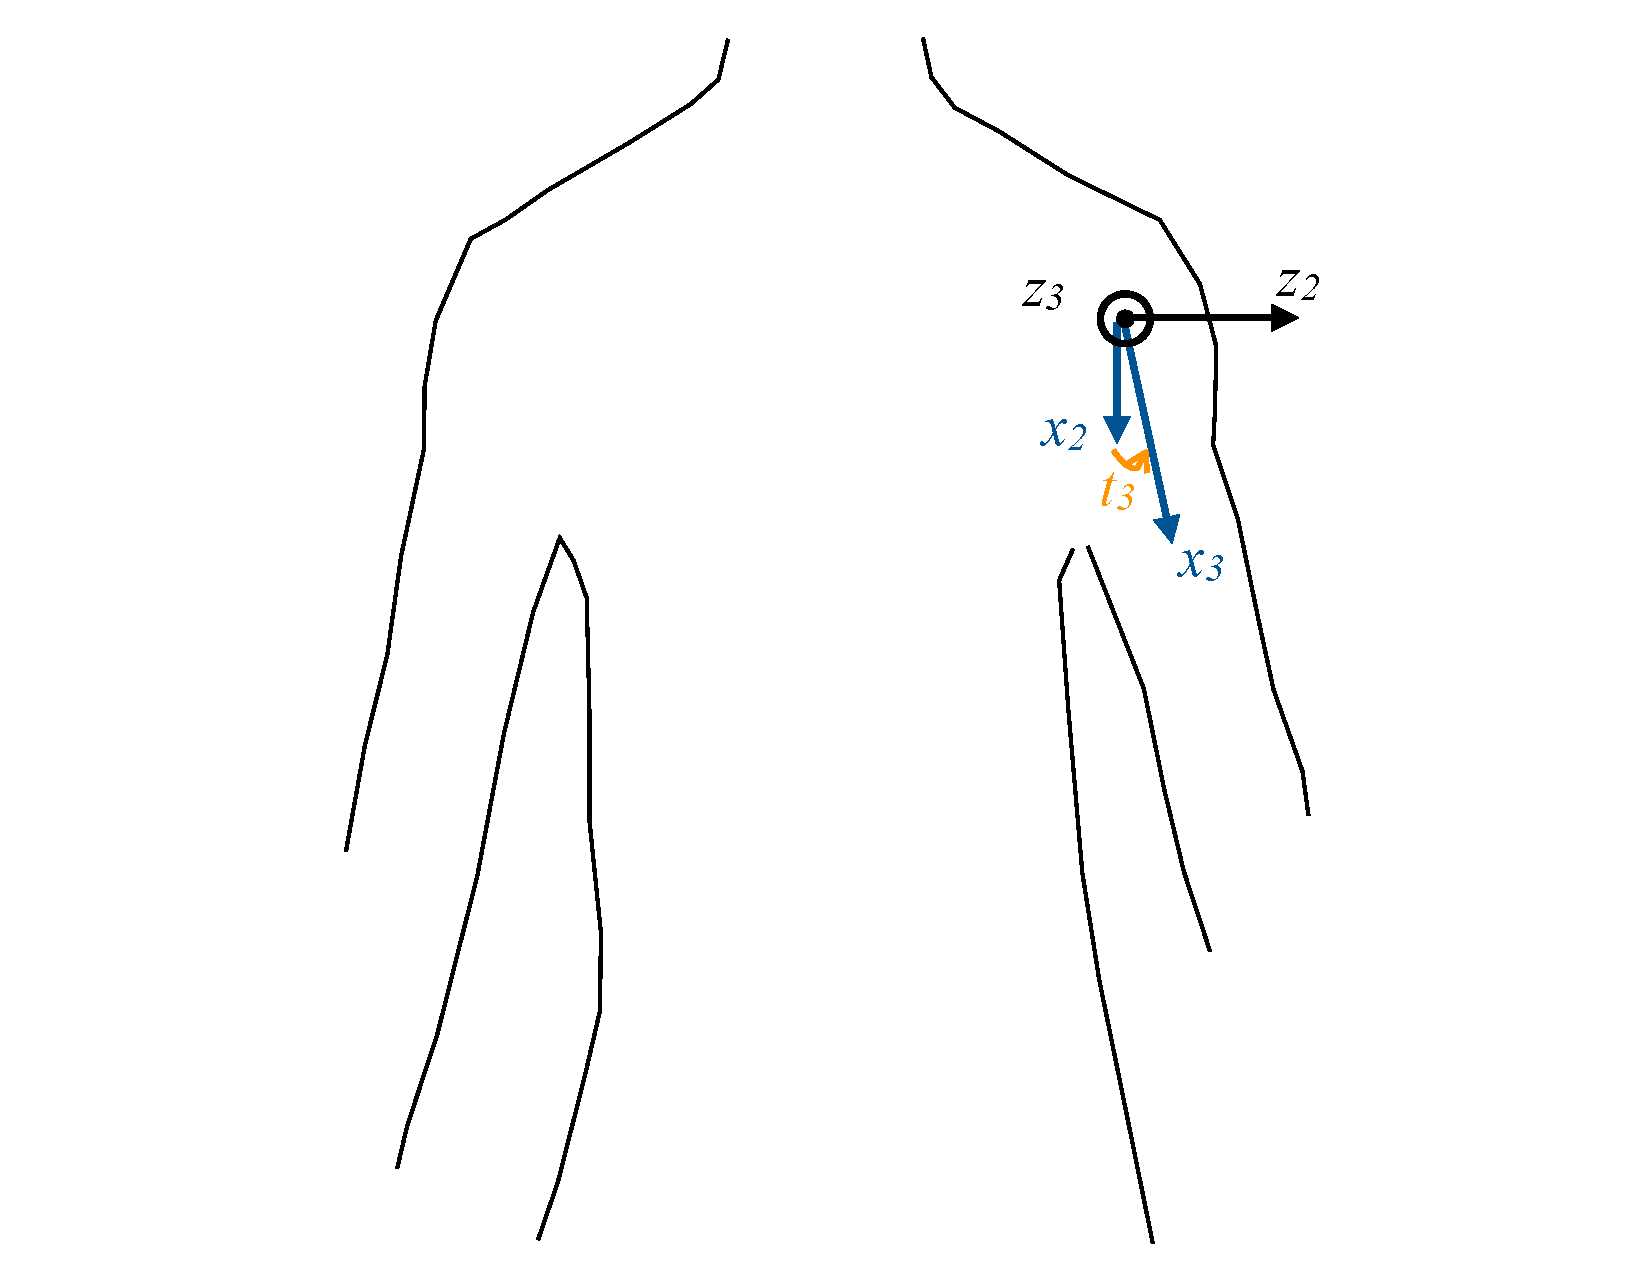
\includegraphics[trim = 50mm 0mm 50mm 0mm, clip, width=\textwidth]{model_3}
        \caption{}
    \end{subfigure}
    ~
    \begin{subfigure}[b]{0.4\textwidth}
        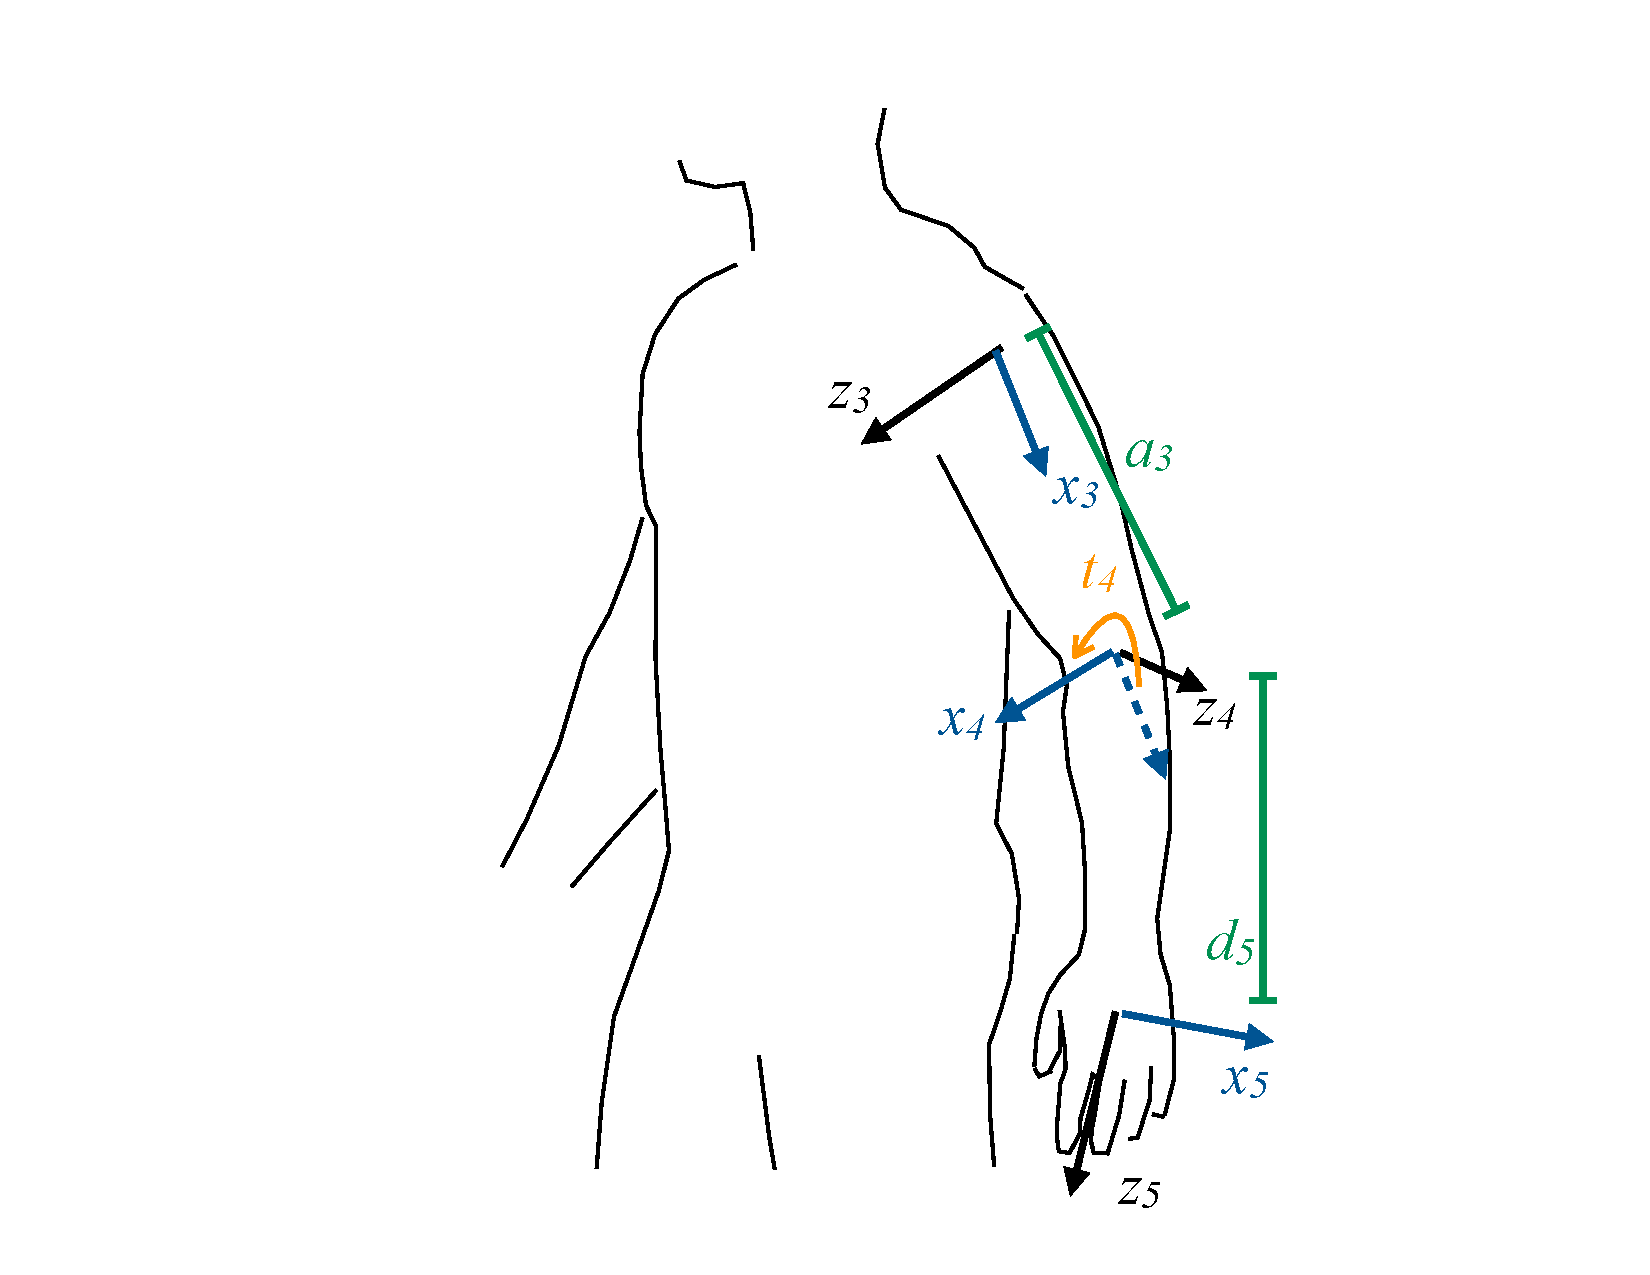
\includegraphics[trim = 50mm 0mm 50mm 0mm, clip, width=\textwidth]{model_4}
        \caption{}
    \end{subfigure}
    \caption{The model of human left arm. $t_i$ stands for $\theta_i$, for $i=1,2,3,4$.}
    \label{fig:model}
\end{figure}



   We carefully specify the linkage model in the following with Fig. \ref{fig:model}. In this kinematic linkage, the hand is chosen to be the end effector, and the base frame is chosen based on the torso (trunk). The origin $O_0$ is set on the shoulder joint. $x_0$ points to the front, and $y_0$ points outward, and $z_0$ points upward. 
   
   
   
   Since the shoulder joint has 3 DOF, we use the first three joints with common origin to model it. The first joint rotates with the axis parallel to spine, and we can use this joint to open or close our chest. The second joint has the rotational axis along the shoulder, and is used to swing the arm forward and backward. The third joint has the rotational axis perpendicular to the surface of the body. The flexibility of rotation in each direction is different; therefore, the plausible degree of each joint is different. 
   
   
   As for the elbow joint, one joint is enough. The origin of the end effector $O_5$ is chosen at the center of the palm, which is exactly the Lao gong acupuncture point in the traditional Chinese medicine. As for the z-axis $z_5$, it is chosen along the direction of fingers. The unit of all frames are chosen to be $1$ cm.
   
   
   % operational space, task
   The human arms are the most dexterous part of the body. They not only account for essential various tasks such as eating, grabbing, etc, they can also perform some social and cultural expressions. We consider the operational space of the arm as the attainable space the hand, which is the front space and the side space mostly.
   
   We define the neutral position as the relaxed position that the arm lays by the body naturally. And one of the standard posture is salute to display respect. In this gesture, the wrist joint is fixed, and the elbow joint and the second joint are involved in this gesture, while the rest of the joints hardly enforce.


%%%%%
\section{Methods}





%%%
\subsection{Denavit-Hartenberg Parameters}


\begin{table}
\begin{center}
   \begin{tabular}{ c | c  c  c  c}
      index $i$ & link length $a_i$ & link twist $\alpha_i$ & link offset $d_i$ & joint angle $\theta_i$ \\ \hline
      0 & 0     & $0$ & \textemdash & \textemdash \\
      1 & 0     & $\pi/2$ & 0 & $\theta_1$ \\
      2 & 0     & $\pi/2$ & 0 & $\theta_2$ \\
      3 & $a_3$ & $3\pi/2$ & 0 & $\theta_3$ \\
      4 & 0     & $3\pi/2$ & 0 & $\theta_4$ \\
      5 & \textemdash & \textemdash & $d_5$ & $3\pi/2$ \\
   \end{tabular}
   \caption{Denavit-Hartenberg Parameters. $a_3$ is the length of upper arm, and $d_5$ is the length of forearm.}
\end{center}
\end{table}


   % joint space
   Since all the joints are revolute, the joint variables can be written as
   \[
      \mathbf{q} = [ \theta_1 \ \theta_2 \ \theta_3 \ \theta_4]^{\mathsf{T}}.
   \]
   By following modified Denavit-Hartenberg conventions, frames will be uniquely determined. The link length $a_3$, which is the length between $z_3$ and $z_4$, is defined to be $36.88$ cm. The link offset $d_5$, which is the length between $x_4$ and $x_5$, is set as $35.92$ cm. The whole Denavit-Hartenberg parameters are listed in Table 1.
   
   With the Denavit-Hartenberg parameters, one can derive the transformation matrix of the frames by
\begin{equation}
   T^{i-1}_i = \begin{pmatrix}
         \cos \theta_i & - \sin \theta_i & 0 & a_{i-1} \\
         \sin \theta_i \cos \alpha_{i-1} & \cos \theta_i \cos \alpha_{i-1} & -\sin \alpha_{i-1} & -d_i \sin \alpha_{i-1} \\
         \sin \theta_i \sin \alpha_{i-1} & \cos \theta_i \sin \alpha_{i-1} & \cos \alpha_{i-1} & d_i \cos \alpha_{i-1} \\
         0 & 0 & 0 & 1 \\
   \end{pmatrix}.
\end{equation}
We have to note that $T_5^4$ is deterministic, while the rest have control parameters as $T_1^0(q_1)$, $T_2^1(q_2)$, $T_3^2(q_3)$, and $T_4^3(q_4)$.





%%%
\subsection{Forward Kinematics}


   We can consider the neutral position with $(\theta_1,\theta_2,\theta_3, \theta_4) = (\pi, 3\pi/2,0,3\pi/2)$. We are interested in the coordinate of the origin of the end effector in the base frame. We can use a series of transformation matrices to get the result. The coordinate of the origin in the end effector in its own frame is $p_5 = (0,0,0)$, the coordinate in the base frame is given by
   \begin{align*}
      p_0 &= T_5^0(\theta_1, \theta_2, \theta_3, \theta_4) \, p_5. \\
          &= T_1^0(\theta_1) \, T_2^1(\theta_2) \, T_3^2(\theta_3) \, T_4^3(\theta_4) \, T_5^4 \, p_5.
   \end{align*}
The implementation is written in the code in \texttt{forward.m}, and we can get the final result as $\texttt{[0 0 -72.80 1]}$, which coincides with our manual calculation.

%%%
\subsection{Inverse Kinematics}


   We try to compute the inverse kinematics of the salute posture with $p_0 = (5, -5, 8)$.
   
   To solve this problem, we use the operation $(q_1,q_2,q_3,q_4)$ to calculate the current position, which can be easily done by forward kinematics. We then use the difference between the desired position and the current position to calculate the next operation. The process is repeated recursively until the norm between the desired position and the current position is no greater than $0.1$.
   
   The adjustment of the operation is the critical part of this algorithm. We use Jacobian matrix between the difference of operations and the difference between positions, as follow
   \begin{equation}
      J = \begin{pmatrix}
         \partial x / \partial \theta_1 & \partial x /\partial \theta_2 & \partial x /\partial \theta_3 & \partial x /\partial \theta_4 \\
         \partial y / \partial \theta_1 & \partial y /\partial \theta_2 & \partial y /\partial \theta_3 & \partial y /\partial \theta_4 \\
         \partial z / \partial \theta_1 & \partial z /\partial \theta_2 & \partial z /\partial \theta_3 & \partial z /\partial \theta_4 \\
   \end{pmatrix},
   \end{equation}
where $x = (T_5^0(\mathbf{q})  p_5)_{1,4}$, $y = (T_5^0(\mathbf{q})  p_5)_{2,4}$ and $z = (T_5^0(\mathbf{q})  p_5)_{3,4}$. Since the Jacobian matrix is a function of operation, we just take the argument as the current operation is each iteration. However, the Jacobian gives the difference of the position to that of the operation, but what we need in the algorithm is the difference of the operation to that of the position. We use the Moore\textendash Penrose pseudoinverse to solve the problem, which is the function \texttt{pinv()} in Matlab. The whole code is in \texttt{inverse.m}.


%%%%%
\section{Results}






%\nocite{*}
%\bibliographystyle{IEEEtran}
%{\small \bibliography{ref}}


\end{document}